% arara: pdflatex
%        File: LinearAlgebra.tex
%     Created: Fri Jun 09 06:00 PM 2023 B
% Last Change: Fri Jun 09 06:00 PM 2023 B
%
\documentclass[12pt, a4paper]{article}

\usepackage[]{amsmath}
\usepackage{amssymb}
\usepackage{amsthm}
\usepackage{mathtools}
\usepackage[]{hyperref}
\usepackage[]{graphicx}
\graphicspath{ {./imgs/} }

% Augmented Matrix (Argument is one less than the number of columns)
\newenvironment{amatrix}[1]{%
  \left(\begin{array}{@{}*{#1}{c}|c@{}}
}{%
  \end{array}\right)
}

\newcommand{\R}{\mathbb{R}}
\newcommand{\spantext}{\text{span}}

\theoremstyle{remark}
\newtheorem{remark}{Remark}
\theoremstyle{definition}
\newtheorem{definition}{Definition}
\newtheorem{example}{Example}
\newtheorem{exercise}{Exercise}

\numberwithin{equation}{section}
\numberwithin{definition}{section}
\numberwithin{example}{section}
\numberwithin{exercise}{section}
\numberwithin{remark}{section}
\numberwithin{figure}{section}
\title{Linear Algebra I \& II Summary}
\author{Paul Kim}
\begin{document}
\maketitle

\section*{Preface}
Note that this is not your actual lecture note,
and I do not condone only sticking to this as your resource.
On the other hand, if you are reading this for your intuition,
you are at the right place.

This document is based on 2019 linear algebra I and 2018 linear algebra II lecture notes by Vicky Neale and Ulrike Tillmann.
You can check them out at \url{https://courses.maths.ox.ac.uk/} in the Archive tab.

Most examples here will include the ones from these lecture notes.

Note that this summary note will gloss over quite many of the proofs, but will try to give geometric intuition behind them.

\newpage
\part{Linear Algebra I}
\newpage

\section{Linear Equations and Matrices}
You've probably already seen linear system of equations like the following:
\begin{align}
    &
    \begin{cases}
        3x + 5y = -1 \\
        4x - y = 10
    \end{cases}
    \label{equ: Linear Equation 1}
    \\
    &
    \begin{cases}
        2x + y = 0 \\
        4x + 2y = 1
    \end{cases}
    \label{equ: Linear Equation 2}
    \\
    &
    \begin{cases}
        8x - 7y + 6z = 59 \\
        x + 2z = 9 \\
        3x + 2y - z = 11
    \end{cases}
    \label{equ: Linear Equation 3}
\end{align}
Note that (\ref{equ: Linear Equation 1}) and (\ref{equ: Linear Equation 3}) are uniquely solvable, but (\ref{equ: Linear Equation 2}) does not have solution.

You've probably also seen examples of ones with infinite solutions (because for example, you have more variables than ``effective'' equations).

You can analyze them by hand, but is there a systematic approach to analyzing them?
Say, you are telling a computer to solve these. What are your options?

\begin{definition}[Matrix]
    For $m,n \geq 1$, an \underline{$m \times n$ matrix} is a rectangular array with $m$ rows and $n$ columns with entries from $\R$ (or $\mathbb{C}$ or other fields).
\end{definition}
\begin{remark}
    \textbf{Always count the number of rows, then number of columns}.
\end{remark}
\begin{remark}
    Notation: For matrix $A \in \R^{m \times n}$, $A_{i,j}$ represents the entry at row $i$ and column $j$.
\end{remark}
\begin{example}[Matrices]
    Here are examples of $3 \times 2$ matrices:
    \begin{align*}
        &
        \begin{pmatrix}
            3 & 2 & 1 \\
            1 & -2/3 & 0
        \end{pmatrix} \\
        &
        \begin{pmatrix}
            0 & 0 & 0 \\
            i & 0 & 0
        \end{pmatrix}
    \end{align*}
\end{example}
\begin{definition}[Vector]
    An $n \times 1$ matrix is called a \textbf{column vector}.
    A $1 \times n$ matrix is called a \textbf{row vector}.
\end{definition}
\begin{example}[Vector]
    Here are examples of a column vector and a row vector respectively:
    \begin{align*}
        &
    \begin{pmatrix}
        1 \\
        0 \\
        -1
    \end{pmatrix}
    \\
    &
    \begin{pmatrix}
        1 & 3 & 2 & 5
    \end{pmatrix}
    \end{align*}
\end{example}
\begin{remark}
    \textbf{I highly recommend using variables for denoting column vectors by default}.
    For example $v = 
    \begin{pmatrix}
        1 \\ 2
    \end{pmatrix}
    $
    If you get a row vector, always denote it with a transpose: $ v^T =
    \begin{pmatrix}
        1 & 2
    \end{pmatrix}
    $
    This is because by convention, we will use left multiplication by a matrix far more often then right multiplication.
\end{remark}
\begin{definition}[Square Matrices]
    A matrix with the same number of rows and columns is called a \textbf{square matrix}.
\end{definition}

\subsection{Matrix Multiplication and Transpose}
Addition and subtractions: $A + B$ are defined naturally by their entry-wise operation. (Note that $A$ and $B$ have to have the same dimensions!)
Multiplication of matrices $A$ and $B$ are defined for $A \in \R^{m \times n}$, $B \in \R^{n \times \ell}$ as the following
\begin{definition}[Matrix Multiplication]
    \begin{equation*}
        \left( A B \right)_{i, j} = \sum_{k = 1}^{n} \left( A_{i,k} \right) \left( B_{k,j} \right)
    \end{equation*}
    Note that the resulting $AB$ has dimension $m \times \ell$.
\end{definition}
\begin{example}[Matrix Multiplication]
    Consider the following two matrices:
    \begin{align*}
        A &=
        \underbrace{
        \begin{pmatrix}
            3 & 1 & 2 \\
            4 & 5 & -1
    \end{pmatrix}}_{2 \times 3} \\
        B &=
        \underbrace{
        \begin{pmatrix}
            10 \\
            15 \\
            -5
        \end{pmatrix}
    }_{3 \times 1}
    \end{align*}
    Then:
    \begin{equation*}
        AB = 
        \underbrace{
        \begin{pmatrix}
            3 & 1 & 2 \\
            4 & 5 & -1
    \end{pmatrix}}_{2 \times 3}
        \underbrace{
        \begin{pmatrix}
            10 \\
            15 \\
            -5
        \end{pmatrix}
    }_{3 \times 1}
    =
    \underbrace{
    \begin{pmatrix}
        3 \times 10 + 1 \times 15 + 2 \times (-5) \\
        4 \times 10 + 5 \times 15 + (-1) \times (-5)
    \end{pmatrix}
}_{2 \times 1}
    \end{equation*}
\end{example}
\begin{remark}
    One way to remember if matrix multiplication is well-defined is to note that:
    $m \times$ \underline{$n$} and \underline{$n$} $\times \ell$ results in $m \times \ell$.
\end{remark}
\begin{remark}
    The way matrix multiplication is defined may not be intuitive.
    However, it is a natural way to capture \textit{linear transforms}.
\end{remark}
\begin{exercise}[Associativity of Matrix Multiplication]
    Show that for $A \in \R^{m \times n}$, $B \in \R^{n \times \ell}$, and $C \in \R^{\ell \times p}$, then $(AB)C = A(BC)$. Is it true that $AB=BA$ in general?
\end{exercise}
\begin{exercise}[Diagonal matrices form a ring]
    Show that for \textbf{diagonal matrices} $A \in \R^{n \times n}$ and $B \in \R^{n \times n}$ such that $A_{i,j} = B_{i,j} = 0$ for $i \neq j$, $AB$ should also be a diagonal matrix.
\end{exercise}
\begin{exercise}[Triangular matrices form a ring]
    Show that for \textbf{upper triangular} $A \in \R^{n \times n}$ and $B \in \R^{n \times n}$ such that $A_{i,j} = B_{i,j} = 0$ for $i > j$, $AB$ should also be an upper triangular matrix.
\end{exercise}
\begin{exercise}
    How many diagonal $A \in \R^{n \times n}$ are there such that
    \begin{equation*}
        A^2 = I
    \end{equation*}
    where $I$ is the \textbf{identity matrix}, a diagonal matrix with only 1s in the diagonal entry.
\end{exercise}
\begin{definition}[Transpose]
    For $A \in \R^{m \times n}$, \textbf{transpose} $A^T \in \R^{n \times m}$ is defined as
    \begin{equation*}
        \left( A^T \right)_{i,j} = A_{j,i}
    \end{equation*}
\end{definition}
\begin{example}[Transpose]
    \begin{equation*}
        \begin{pmatrix}
            3 & 0 & 1 \\
            4 & 2 & 5
        \end{pmatrix}^T
        =
        \begin{pmatrix}
            3 & 4 \\
            0 & 2 \\
            1 & 5
        \end{pmatrix}
    \end{equation*}
\end{example}
\begin{remark}
    \begin{itemize}
            \item Taking transpose of a row vector turns it into a column vector.
            \item Taking a transpose of a column vector turns it into a row vector.
            \item For any $A \in \R^{m \times n}$, $\left( A^T \right)^T = A$
    \end{itemize}
\end{remark}
\begin{exercise}[Symmetric Triangular Matrix is Diagonal]
    Show that if an upper triangular matrix $A \in \R^{n \times n}$ satisfies $A^T = A$, then it must be a diagonal matrix.
\end{exercise}
\begin{exercise}[Antisymmetric Matrix Does Not Have Diagonal Entries]
    Show that if $A \in \R^{n \times n}$ satisfies $A^T = -A$, then $A_{i,i} = 0$ for all $i = 1, \cdots n$.
\end{exercise}
\begin{exercise}[Transpose of Product of Matrix]
    Show that for any $A \in \R^{m \times n}$ and $B \in \R^{n \times \ell}$,
    \begin{equation*}
        \left( AB \right)^T = B^T A^T
    \end{equation*}
    Using this result, show that product of two symmetric matrices ($A^T = A$) is also a symmetric matrix.
\end{exercise}
\begin{remark}
    For two column vectors $v_1$ and $v_2$, the dot product can be written as $v_1^T v_2$.
    This becomes a useful notation for dot product, in factf
    \footnote{
    Technically $1 \times 1$ matrix, but there is no problem in taking that as just a scalar.}
\end{remark}

\section{System of Simultaneous Linear Equations to Matrix Equations}
We've seen a system like (\ref{equ: Linear Equation 1}), (\ref{equ: Linear Equation 2}), and (\ref{equ: Linear Equation 3}).

We can turn the three examples of linear system of equations to the following \textbf{matrix equations} of the form $\underbrace{A}_{\text{Matrix}}\underbrace{x}_{\text{Column Vector}} = \underbrace{b}_{\text{Column Vector}}$:
\begin{align}
    &
    \begin{pmatrix}
        3 & 5 \\
        4 & -1
    \end{pmatrix}
    \begin{pmatrix}
        x \\ y
    \end{pmatrix}
    &=
    \begin{pmatrix}
        -1 \\ 10
    \end{pmatrix}
    \\
    &
    \begin{pmatrix}
        2 & 1 \\
        4 & 2
    \end{pmatrix}
    \begin{pmatrix}
        x \\ y
    \end{pmatrix}
    &= 
    \begin{pmatrix}
        0 \\ 1
    \end{pmatrix}
    \\
    &
    \begin{pmatrix}
        8 & -7 & 6 \\
        1 & 0 & 2 \\
        3 & 2 & -1
    \end{pmatrix}
    \begin{pmatrix}
        x \\ y \\ z
    \end{pmatrix}
    &=
    \begin{pmatrix}
        59 \\ 9 \\ 11
    \end{pmatrix}
\end{align}

One could do even better and skip writing the name of the variables:
\begin{align}
    &
    \begin{amatrix}{2}
        3 & 5 & -1 \\
        4 & -1 & 10
    \end{amatrix}
    \\
    &
    \begin{amatrix}{2}
        2 & 1 & 0 \\
        4 & 2 & 1
    \end{amatrix}
    \\
    &
    \begin{amatrix}{3}
        8 & -7 & 6 & 59 \\
        1 & 0 & 2 & 9 \\
        3 & 2 & -1 & 11
    \end{amatrix}
\end{align}
(the bar is decorative to show that the system is augmented.)

Our task is to solve it, that is, we wish to put $\left( A \middle| b \right)$ into the form $\left( I \middle| \tilde b \right)$.
This is unfortunately not possible to do\footnote{
A colloquial saying is that with $n$ variables to solve, you need $n$ independent equations.}.

For example, the following system is over-determined (more equations\footnote{Conditions} than variables):
\begin{equation*}
    \begin{cases}
    3x + y = -4 \\
    2x - 5y = 3 \\
    x + 2y = 8
    \end{cases}
\end{equation*}
and the following is under-determined (less equations than variables):
\begin{equation*}
    \begin{cases}
        x + 2y = 5
    \end{cases}
\end{equation*}
Also (\ref{equ: Linear Equation 2}) is an inconsistent system, as the two equations violate each other.
As you could see, \underline{there are many ways things can go wrong}.

A systematic approach to make analysis easier by performing ``row operations'' is the \textbf{Gaussian elimination}.

\section{EROs and Gaussian Elimination}
\begin{definition}[Elementary Row Operations (ERO)]
    For a matrix $A \in \R^{m \times n}$, following are the three elementary row operations.
    \begin{itemize}
        \item For $1 \leq r < s \leq m$, $R_s \leftrightarrow R_r$ (Exchange row $r$ and row $s$)
        \item For $1 \leq r \leq m$ and $\lambda \neq 0$, $R_r \rightarrow \lambda R_r$ (Multiply row $r$ by $\lambda$)
        \item For $1 \leq r, s \leq m$ where $r \neq s$ and $\lambda \in \mathbb{F}$, $R_s \rightarrow R_s + \lambda R_r$ (Add to row $s$ the row $r$ multiplied by $\lambda$)
    \end{itemize}
\end{definition}
\begin{remark}
    It is \textbf{paramount} that each operation is reversible.
\end{remark}
\begin{remark}
    It is \textbf{recommended} that you do not compose bunch of EROs as one ERO, as tempting as it is.
    Using pure EROs is useful for determinant analysis later.
\end{remark}
Now we need the notion of ``simplified'' matrix under these operations.
\begin{definition}[Echelon Form]
    $M \R^{m \times n}$ is in \textbf{echelon form} if
    \begin{itemize}
        \item If row $r$ of $M$ has any nonzero entries, the first of these is 1.
        \item If $1 \leq r < s \leq m$, and row $r$ and row $s$ contain nonzero entries ($M_{r,j}$ and $M_{s, k}$ respectively), then $j < k$.
            \begin{itemize}
                \item ``Leading entry of lower rows should come to the right of the ones on the higher rows.''
            \end{itemize}
        \item If row $r$ of $M$ contains nonzero entries and row $s$ does not, then $r < s$
            \begin{itemize}
                \item ``Zero rows are below all nonzero rows.''
            \end{itemize}
    \end{itemize}
\end{definition}
\begin{example}[Echelon Form]
    The following matrix in echelon form:
    \begin{equation*}
        \begin{pmatrix}
            1 & 2 & 3 & 4 & 2 \\
            0 & 1 & 2 & 3 & 0 \\
            0 & 0 & 0 & 0 & 1
        \end{pmatrix}
    \end{equation*}
\end{example}
\subsection{Gaussian Elimination}
Now we need an algorithm to perform Gaussian elimination to reduce matrix.
The idea is to take a matrix $A$, and eliminate the leading order entries one by one to echelon form.
\begin{example}[Gaussian Elimination]
    \begin{align*}
        \begin{amatrix}{2}
            3 & 5 & -1 \\
            4 & -1 & 10
        \end{amatrix}
        & \xrightarrow{\substack{R_1 \rightarrow \frac{1}{3} R_1 \\ R_2 \rightarrow \frac{1}{4} R_2}}
        \begin{amatrix}{2}
            1 & \frac{5}{3} & -\frac{1}{3} \\
            1 & -\frac{1}{4} & \frac{5}{2}
        \end{amatrix}
        \\
        & \xrightarrow{R_2 \rightarrow R_2 - R1}
        \begin{amatrix}{2}
            1 & \frac{5}{3} & -\frac{1}{3} \\
            0 & -\frac{23}{12} & \frac{17}{6}
        \end{amatrix} \\
        & \xrightarrow{R_2 \rightarrow -\frac{12}{23}R_2}
        \underbrace{
        \begin{amatrix}{2}
            1 & \frac{5}{3} & -\frac{1}{3} \\
            0 & 1 & -\frac{34}{23}
    \end{amatrix}}_{\text{echelon}}
    \end{align*}
\end{example}
\begin{remark}
    If there was a zero in the leading entry of the first column, one could swap the rows.
\end{remark}
\begin{example}[Gaussian Elimination (Cont'd)]
    We could take it even further and get \textbf{reduced row echelon (RRE) form}.
    \begin{align*}
        \begin{amatrix}{2}
            1 & \frac{5}{3} & -\frac{1}{3} \\
            0 & 1 & -\frac{34}{23}
        \end{amatrix}
        & \xrightarrow{R_1 \rightarrow R_1 - \frac{5}{3}R_2}
        \underbrace{
        \begin{amatrix}{2}
            1 & 0 & -\frac{49}{23} \\
            0 & 1 & \frac{34}{23}
    \end{amatrix}}_{\text{RRE}}
    \end{align*}
    So $x = -\frac{49}{23}$ and $y = \frac{34}{23}$ for (\ref{equ: Linear Equation 1}).
\end{example}
\begin{exercise}
    Given $A \in \R^{n \times n}$, show that it can be reduced to RRE within $n^2$ EROs.
\end{exercise}
\subsection{Inverse Matrix}
\begin{definition}[Inverse Matrix]
    Note that if it is possible to identify $B \in \R^{n \times n}$ such that $AB = BA = I$, then we call this $B$ the \textbf{inverse matrix} of $A$, and write $A^{-1} \coloneqq B$.
    We also say that $A$ is invertible in this case.
\end{definition}
\begin{remark}
    For a well-posed matrix equation $Ax = b$ where $A \in \R^{n \times n}$ being an invertible matrix,
    one could write the solution as $x = A^{-1} b$.
\end{remark}
\begin{exercise}[Inverse is Unique]
    If $A \in \R^{n \times n}$ is invertible, show that the inverse $A^{-1}$ is well-defined.
\end{exercise}
\begin{exercise}[Inverse of Product]
    If $A,B \in \R^{n \times n}$ are both invertible matrices, then show that
    \begin{equation*}
        \left( AB \right)^{-1} = B^{-1}A^{-1}
    \end{equation*}
\end{exercise}
\begin{exercise}[Inverse Transpose]
    If $A \in \R^{n \times n}$ is invertible, then show that $A^{T}$ is also invertible,
    and that:
    \begin{equation*}
        \left( A^T \right)^{-1} = \left( A^{-1} \right)^T
    \end{equation*}
\end{exercise}
\begin{remark}
    The above exercise shows that one could write $A^{-T}$ as a shorthand for inverse transpose of $A$.
\end{remark}
It is possible to compute the inverse matrix (should it exist) via Gaussian elimination.
Consider $A \in \R^{n \times n}$, an invertible matrix.
Perform Gaussian elimination on $\left( A \middle| I \right) \in \R^{n \times 2n}$, then we should end up with:
$\left( I \middle| A^{-1} \right)$.
\begin{remark}
    For the proof, refer to the actual lecture note. Try showing that if $A \in \R^{n \times n}$ is invertible, then RRE is the identity matrix.
\end{remark}
\begin{remark}
    In practice, computing the inverse matrix is in fact not a feasible thing to do (considering data sets are enormous, and we are often only interested in solution to one single solution to a matrix equation).
\end{remark}
\section{Vector Spaces}
\begin{definition}[Vector Space]
    Let $\mathbb{F}$ be a field. A \textbf{vector space} over $\mathbb{F}$ is a non-empty set $V$ with
    addition and scalar multiplication operation defined, satisfying the vector space axioms:
    \begin{itemize}
        \item Addition is commutative.
            \begin{itemize}
                \item $u + v = v + u$.
            \end{itemize}
        \item Addition is associative.
            \begin{itemize}
                \item $\left( u + v \right) + w = u + \left( v + w \right)$
            \end{itemize}
        \item There exists an additive identity.
            \begin{itemize}
                \item $0 \in V$
            \end{itemize}
        \item There exists additive inverse for every element.
            \begin{itemize}
                \item $\forall v \in V: \exists (-v) \in V$
            \end{itemize}
        \item Scalar multiplication is distributive over vector addition.
            \begin{itemize}
                \item $\lambda \left( u + v \right) = \lambda u + \lambda v$
            \end{itemize}
        \item Scalar multiplication is distributive over scalar multiplication.
            \begin{itemize}
                \item $\left( \lambda + \mu \right) v = \lambda v + \mu v$
            \end{itemize}
        \item Scalar multiplication interacts well with field multiplication.
            \begin{itemize}
                \item $\left( \lambda \mu \right) v = \lambda \left( \mu v \right)$
            \end{itemize}
        \item Identity for scalar multiplication.
            \begin{itemize}
                \item $1v = v$
            \end{itemize}
    \end{itemize}
\end{definition}
\begin{example}[Vector Space: $\R^n$]
    $\R^n$ is a vector space.
    Honestly, this is the most important vector space, so I suggest you get used to working in here.
    Note that often you can restrict your attention to $\R^3$, and most of your intuition also applies in higher dimensions.
\end{example}
\begin{example}[Other Vector Spaces]
    Other vector spaces include:
    \begin{itemize}
        \item $\mathbb{C}$ is a vector space over field $\R$ (essentially $\mathbb{C}$ is the same thing as $\R^2$).
        \item $\mathcal{P}_n$, the space of polynomials of degree $n$ or less is a vector space over $\R$.
    \end{itemize}
\end{example}
\begin{exercise}[Uniqueness of Additive Identity and Inverse]
    For vector space $V$, 
    \begin{itemize}
            \item show that the additive identity element is unique.
            \item show that for any $v \in V$, the additive inverse $(-v)$ is well-defined.
    \end{itemize}
\end{exercise}
\begin{definition}[Subspaces]
    Let $V$ be a vector space over $\mathbb{F}$. $U \subset V$ is a \textbf{subspace} of $V$ if it is nonempty, closed under addition and scalar multiplication.
\end{definition}
\begin{exercise}[Subspace Test]
    Let $V$ be a vector space over $\mathbb{F}$.
    Let $U$ be a subset of $V$.
    Show that $U$ is a subspace of $V$ if and only if $0 \in U$ and $\lambda u_1 + u_2 \in U$ for all $u_1, u_2 \in U$ and $\lambda \in \mathbb{F}$.
\end{exercise}
\begin{remark}
    If you think about subspace test for a long time, it kinda becomes obvious; the fact that $\lambda u_1 + u_2 \in U$ captures the idea of closure under both addition and scalar multiplication.
\end{remark}
\begin{exercise}[Subspace is also a Vector Space]
    If $V$ is a vector space and $U$ is a subspace of $V$,
    show that
    \begin{itemize}
        \item $U$ is a vector space.
        \item If $W$ is a subspace of $U$, then $W$ is a subspace of $V$.
    \end{itemize}
\end{exercise}
\begin{example}[Hyperplane is a Subspace of $\R^n$]
    $U \coloneqq \left\{ \left( x,y,z \right) \in \R^3 \middle| x + 2y + z = 0\right\} \leq \R^3$.
    \begin{figure}[h]
        \centering
        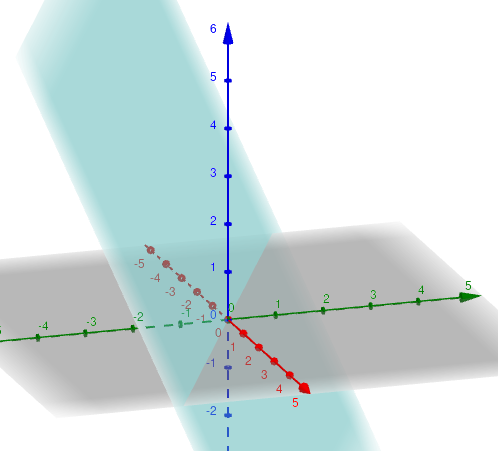
\includegraphics[scale=0.2]{hyperplane121}
        \caption{$x + 2y + z = 0$}
    \end{figure}
\end{example}
\begin{definition}[Sum Space]
    For $A,B \subset V$ where $V$ is a vector space, define $A + B \coloneqq \left\{ a + b \middle| a\in A, b \in B \right\}$
\end{definition}
\begin{exercise}[Sum Space and Intersection are Subspaces]
    For $V$ vector space, and $U,W \leq V$, show that
    \begin{itemize}
        \item $U + W$ is a subspace of $V$.
        \item $U \cap W$ is a subspace of $V$.
    \end{itemize}
    Construct an example where $U \cup W$ is not a subspace.
\end{exercise}

\section{Bases}
\begin{definition}[Span]
    \textbf{Span} of vectors $v_1, v_2, \cdots, v_k$ is defined as $\spantext \left( \left\{ v_1, \cdots, v_k \right\} \right) \coloneqq  \left\{ \sum_{i=1}^k a_iv_i \middle| a_i \in \mathbb{F} \right\}$.
\end{definition}
\begin{example}[Span]
    Span of $\left\{ e_1, e_2 \right\}$ is $\R^2$, where $e_i$ are $i$\textsuperscript{th} canonical vector.
    Span of $\left\{ 
        \begin{pmatrix}
            1 \\ 1
        \end{pmatrix},
        \begin{pmatrix}
            1 \\ -1
        \end{pmatrix}
    \right\}$ is also $\R^2$.
\end{example}
\begin{exercise}[Span is Subspace]
    Show that span of finite number of vectors is a subspace.
\end{exercise}
\begin{definition}[Linear Combination]
    $u$ is a \textbf{linear combination} of $v_1, \cdots, v_k$ if $u \in \spantext \left( \left\{ v_1, \cdots, v_k \right\} \right)$
\end{definition}
\end{document}


